\documentclass[14pt,a4paper]{extarticle}
\usepackage{amsmath}
\usepackage{graphicx}
\usepackage[utf8]{inputenc}    
\usepackage[T2A]{fontenc}
\usepackage[russian]{babel}
\usepackage{setspace}
\usepackage{geometry}
\usepackage{longtable}
\usepackage{makecell}
\usepackage{listings}
\usepackage{xcolor} 
\geometry{
    left=3cm,
    right=1.5cm,
    top=2cm,
    bottom=2cm
}

\begin{document}
\thispagestyle{empty}

\begin{center}
САНКТ-ПЕТЕРБУРГСКИЙ ГОСУДАРСТВЕННЫЙ УНИВЕРСИТЕТ\\
МАТЕМАТИКО-МЕХАНИЧЕСКИЙ ФАКУЛЬТЕТ\\
КАФЕДРА ФИЗИЧЕСКОЙ МЕХАНИКИ
\end{center}

\vspace{4cm}

\begin{center}
\textbf{Методы измерений и электромеханические системы}\\
\vspace{0.5cm}
Отчёт по лабораторной работе №1
\end{center}

\vspace{0.5cm}

\begin{center}
\textbf{«Обработка результатов физических измерений. Вариант в. Измерение сопротивлений резисторов с помощью моста универсального E7-4 »}
\end{center}

\vspace{4cm}

\begin{flushright}
Выполнил студент:\\
Тузова Анастасия Александровна\\
группа: 24.Б51-мм

\vspace{1.5cm}

Проверил:\\
к.ф.-м.н., доцент\\
Кац Виктор Михайлович
\end{flushright}

\vfill

\begin{center}
Санкт-Петербург, 2026 г.
\end{center}
\newpage   
\tableofcontents 
\newpage
\section{Введение}
\subsection{Цель работы}
Практическое освоение методики прямых многократных измерений физической величины с помощью универсального моста Е7-4 и первичная статистическая обработка результатов наблюдений.

\subsection{Решаемые задачи}
\begin{enumerate}
    \item Освоить методику использования измерительного прибора для многократного прямого измерения физической величины.
    \item Выполнить простейшую статистическую обработку серии результатов наблюдений при прямых измерениях.
\end{enumerate}
\newpage
\section{Основная часть}
\subsection{Теоретическая часть}
\textbf{Вычисление погрешности прибора \(\Delta R_{\text{приб}}\):}

\begin{equation}
\Delta R_{\text{приб}} = \frac{\delta \cdot R_{\text{ср}}}{100\%},
\end{equation}

\begin{equation}
\delta = \pm \left( 2 + \frac{9}{R_{\text{ср}}} \right) \% = \frac{\Delta R_{\text{приб}}}{R_{\text{ср}}} \cdot 100\%,
\end{equation}

\begin{equation}
R_{\text{ср}} = \frac{\sum R_i}{n}.
\end{equation}
где: \(\delta\) — относительная погрешность измерения в \%  
\\Среднеквадратичное отклонение:
\[
\sigma \approx \sqrt{\frac{\sum (R_i - R_{\text{cp}})^{2}}{n-1}} 
\]
Средняя квадратичная погрешность среднего: \( \Delta R \approx \sigma / \sqrt{n} \)
\subsection{Эксперимент}
\begin{figure}[h!]
    \centering
   \includegraphics[width=0.8\textwidth, trim=2cm 15cm 2cm 5cm, clip]{img1.PDF}
    \caption{Схема установки}
    \label{fig:img1}
\end{figure}
\newpage
\begin{figure}[h!]
    \centering
    \includegraphics[width=0.8\textwidth,clip]{most.jpg}
    \caption{Фото установки}
    \label{fig:most.jpg}
\end{figure}
\newpage
\subsection{Обработка данных и обсуждение результатов}
\subsubsection*{Исходный код}
Составим таблицу, вычисляющую отклонения от среднего и квадратичные отклонения в помощью C++
\begin{lstlisting}[language=C++]
#include<iostream>
#include <fstream>
#include <iomanip>
int main() {
	double a[50];
	for (int i = 0; i < 50; ++i) {
		std::cin >> a[i];
	}
	double s = 0;
	for (int i = 0; i < 50; ++i) {
		s+=a[i];
	}
	s = s / 50;

    std::ofstream file3("table.txt");
    file3 << std::fixed << std::setprecision(6);
    file3 << "#\\tR_i\t\td_i\t\td_i^2" << std::endl;
	double p = 0;
	double y = 0;
    for (int i = 0; i < 50; ++i) {
        double d = a[i] - s;
		p += abs(d);
		y += d * d;
        file3 << i + 1 << "\t" << a[i] << "\t\t" << d
        << "\t\t"  << d * d << std::endl;
    }
	file3 << s;
	file3 << "\n";
	file3 << p;
	file3 << "\n";
	file3 << y;
    file3.close();
    return 0;
}
\end{lstlisting}
\addcontentsline{toc}{subsubsection}{Исходный код}
\newpage
\subsubsection*{Таблицы}
1) Измерения на грубой шкале
{\small

\setlength{\tabcolsep}{4pt}  % уменьшаем отступы в ячейках
\begin{longtable}{|c|c|c|c|}
\caption{Результаты измерений}
\label{tab:resul}\\
\hline
Номер п.п. & \makecell{Диапазон,\\(Ом)} & \makecell{\(R_i\)\\(Oм)} & \makecell{\(\Delta R_{\text{приб}}\)\\(Oм)} \\
\hline
\endfirsthead

\multicolumn{4}{c}{{\tablename\ \thetable{} — продолжение}} \\
\hline
Номер п.п. & Диапазон, Ом & \(U_i\), В & \(\Delta U_{\text{приб}}\), В \\
\hline
\endhead

\hline
\multicolumn{4}{|r|}{продолжение на следующей странице} \\
\endfoot

\hline
\endlastfoot

1  & 0–10 & 4.00 & ±0,17 \\
2  & 0–10 & 4.00 & ±0,17 \\
3  & 0–10 & 4.00 & ±0,17 \\
4  & 0–10 & 4.00 & ±0,17 \\
5  & 0–10 & 4.00 & ±0,17 \\
6  & 0–10 & 4.00 & ±0,17 \\
7  & 0–10 & 4.00 & ±0,17 \\
8  & 0–10 & 4.00 & ±0,17 \\
9  & 0–10 & 4.00 & ±0,17 \\
10 & 0–10 & 4.00 & ±0,17\\

\end{longtable}
}
Получим \( R_{\text{ср}} = 4,00 \, \text{Oм} \)



2) Измерения на точной шкале
\begin{itemize}
    \item Диапазон показаний прибора \( 0 - 1 \, \text{Oм} \)
    \item Погрешность прибора \( \Delta R_{\text{приб}} = \pm 0{,}1694 \, \text{Ом} \)
\end{itemize}
{
\setlength{\tabcolsep}{6pt}
\begin{longtable}{|c|c|c|c|}
\caption{Результаты измерений и их обработка}
\label{tab:res}\\
\hline
№ & \makecell{\(R_i\)\\Ом} & \makecell{\(d_i\)\\Ом} & \makecell{\(d_i^2\)\\Ом\(^2\)} \\
\hline
\endfirsthead

\multicolumn{4}{c}{{\tablename\ \thetable{} — продолжение}} \\
\hline
№ & \(R_i\), Ом & \(d_i\), Ом & \(d_i^2\), Ом\(^2\) \\
\hline
\endhead

\hline

\endfoot

\hline
\endlastfoot

1  & 4.11 & 0.1412 & 0.019937 \\
2  & 4.05 & 0.0812 & 0.006593 \\
3  & 4.00 & 0.0312 & 0.000973 \\
4  & 3.98 & 0.0112 & 0.000125 \\
5  & 4.01 & 0.0412 & 0.001697 \\
6  & 4.00 & 0.0312 & 0.000973 \\
7  & 3.99 & 0.0212 & 0.000449 \\
8  & 3.95 & -0.0188 & 0.000353 \\
9  & 3.92 & -0.0488 & 0.002381 \\
10 & 3.97 & 0.0012 & 0.000001 \\
11 & 3.92 & -0.0488 & 0.002381 \\
12 & 3.96 & -0.0088 & 0.000077 \\
13 & 3.97 & 0.0012 & 0.000001 \\
14 & 3.95 & -0.0188 & 0.000353 \\
15 & 3.92 & -0.0488 & 0.002381 \\
16 & 3.94 & -0.0288 & 0.000829 \\
17 & 4.03 & 0.0612 & 0.003745 \\
18 & 3.99 & 0.0212 & 0.000449 \\
19 & 4.01 & 0.0412 & 0.001697 \\
20 & 4.02 & 0.0512 & 0.002621 \\
21 & 3.93 & -0.0388 & 0.001505 \\
22 & 3.95 & -0.0188 & 0.000353 \\
23 & 3.92 & -0.0488 & 0.002381 \\
24 & 3.94 & -0.0288 & 0.000829 \\
25 & 3.97 & 0.0012 & 0.000001 \\
26 & 3.91 & -0.0588 & 0.003457 \\
27 & 3.99 & 0.0212 & 0.000449 \\
28 & 3.91 & -0.0588 & 0.003457 \\
29 & 3.94 & -0.0288 & 0.000829 \\
30 & 4.00 & 0.0312 & 0.000973 \\
31 & 3.98 & 0.0112 & 0.000125 \\
32 & 3.95 & -0.0188 & 0.000353 \\
33 & 3.93 & -0.0388 & 0.001505 \\
34 & 3.98 & 0.0112 & 0.000125 \\
35 & 3.92 & -0.0488 & 0.002381 \\
36 & 3.96 & -0.0088 & 0.000077 \\
37 & 4.03 & 0.0612 & 0.003745 \\
38 & 4.00 & 0.0312 & 0.000973 \\
39 & 4.03 & 0.0612 & 0.003745 \\
40 & 3.90 & -0.0688 & 0.004733 \\
41 & 3.94 & -0.0288 & 0.000829 \\
42 & 3.99 & 0.0212 & 0.000449 \\
43 & 3.98 & 0.0112 & 0.000125 \\
44 & 3.91 & -0.0588 & 0.003457 \\
45 & 4.01 & 0.0412 & 0.001697 \\
46 & 3.90 & -0.0688 & 0.004733 \\
47 & 3.95 & -0.0188 & 0.000353 \\
48 & 4.00 & 0.0312 & 0.000973 \\
49 & 3.95 & -0.0188 & 0.000353 \\
50 & 3.98 & 0.0112 & 0.000125 \\
\hline
\multicolumn{2}{|c|}{\(R_{\text{ср}} = \dfrac{\sum_{i=1}^{50} R_i}{50} = 3.9698\) Ом} & 
\(\sum |d_i| = 1.762400
\) Ом & 
\(\sum d_i^2 = 0.093128\) Ом\(^2\) \\
\hline
\end{longtable}
}
Среднеквадратичное отклонение:
\[
\sigma \approx \sqrt{\frac{\sum (R_i - R_{\text{cp}})^{2}}{n-1}} = 0.0436~\text{Ом}
\]
\( \sigma_{\bar{x}} \approx \dfrac{\sigma}{\sqrt{50}} = 0{,}00617~\text{Ом} \)

\[
x = \overline{x} \pm \Delta x
\]
\[
R = 3{,}9698 \pm 0.0062~\text{Ом}
\]
Предел погрешности  \(\omega\) < < предела допускаемой погрешности прибора.
\\\textbf{Следовательно погрешность измерений равна инструментальной погрешности - пределу допускаемой погрешности прибора.}
\[
R_{\text{min}} = 3.89~\text{Ом},\quad R_{\text{max}} = 4.11~\text{Ом}
\]
Округляем, получаем диапазон от 3.89 до 4.13 Ом. Разобьем диапазон (24~Ом) на 8 интервалов по 0,3~Ом.
\\Составим таблицу данных для построения гистограммы и графика.
\begin{table}[ht!]
\centering
\caption{Результаты измерений}
\label{tab:results}
\small
\begin{tabular}{|c|c|c|c|}
\hline
Номер интервала & Границы интервалов, Ом & Число случаев $\Delta n$ & Доля $\delta n = \Delta n / n$ \\
\hline
1  & 3.89–3.92 & 4  & 0.04 \\
2  & 3.92–3.95 & 10 & 0.20 \\
3  & 3.95–3.98 & 12 & 0.24 \\
4  & 3.98–4.01 & 12 & 0.24 \\
5  & 4.01–4.04 & 9  & 0.18 \\
6  & 4.04–4.07 & 4  & 0.08 \\
7  & 4.07–4.10 & 0  & 0.00 \\
8  & 4.10–4.13 & 1  & 0.02 \\
\hline
\multicolumn{3}{|c|}{$n = \sum \Delta n = 50$} & $\dfrac{\sum \Delta} n = 1.000$ \\
\hline
\end{tabular}
\end{table}
\addcontentsline{toc}{subsubsection}{Таблицы}
\newpage
\subsubsection*{Графики}
\begin{figure}[h!]
    \centering
   \includegraphics[width=0.8\textwidth, clip]{output1.png}
    \caption{Зависимость результатов наблюдений от времени(для грубой шкалы)}
    \label{fig:output1}
\end{figure}
\begin{figure}[h!]
    \centering
   \includegraphics[width=0.8\textwidth, clip]{output.png}
    \caption{Зависимость результатов наблюдений от времени(для точного случая)}
    \label{fig:output}
\end{figure}
\begin{figure}[h!]
    \centering
   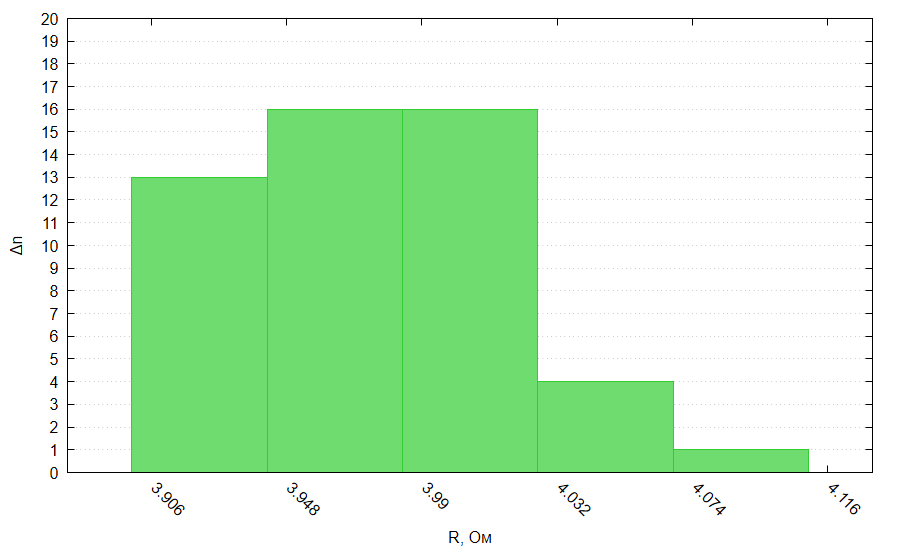
\includegraphics[width=0.8\textwidth, clip]{plot2_histogram.png}
    \label{fig:output3}
\end{figure}
\begin{figure}[ht!]
    \centering
   \includegraphics[width=0.8\textwidth, clip]{plot3_spline_freq.png}
    \caption{Распределение результатов наблюдений: график зависимости}
    \label{fig:output2}
\end{figure}
Для любого распределения (исходя из графика) можно грубо оценить:
\[
\sigma \approx |R_{\text{пик}} - R_{\text{перегиба}}| \approx |4.02 - 3.98|~\text{Ом} 
\]

\[
\sigma \approx 0.04 ~\text{Ом}
\]

\addcontentsline{toc}{subsubsection}{Графики}
\newpage
\section{Выводы}
В результате проделанной работы я ознакомилась с методиками использования измерительного прибора для многократного прямого измерения физической величины на примере работы с универсальным мостом E7-4 (измерение сопротивления резисторов), выполнила простую статистическую обработку серии результатов наблюдений при прямых измерениях, вычислила дисперсию и среднеквадратичное отклонение. Сравнила значение средней квадратичной погрешности измерений и погрешности прибора. Научилась с помощью графика определять дисперсию.
\newpage
\section{Список литературы}
\begin{enumerate}
    \item GitHub.-2026. https://github.com/tuzova-aa/Workshop1.git
\end{enumerate}
\end{document}
